\documentclass[12pt]{article}
\usepackage{amsmath}
\setlength{\jot}{2ex}
\usepackage{mathrsfs}
\usepackage{steinmetz}
\usepackage{graphicx}
\usepackage{wrapfig}
\usepackage{booktabs}
\usepackage[letterpaper, margin=1in]{geometry}
\usepackage{fancyhdr}
\pagestyle{fancy}
\fancyhead[R]{Chapter 9 Problems}
\fancyfoot[C]{\thepage}
\renewcommand{\headrulewidth}{1pt}
\renewcommand{\footrulewidth}{1pt}
\usepackage [autostyle, english = american]{csquotes}
\MakeOuterQuote{"}
\renewcommand{\baselinestretch}{1.0}
\newcommand{\objects}[2]{%
  \leavevmode\vbox{\hbox{#1}\nointerlineskip\hbox{#2}}%
}
\begin{document}
    \section*{Problem 9.3}
    At $t = -2\ ms$, a sinusoidal voltage is known to be zero and going positive.
    The voltage is next zero at $12\ ms$. It is also known tat the voltage is
    $80.9\ V$ at $t = 0$. \\
    \textbf{What is the frequency of $v(t)$ in hertz?}
    \begin{gather*}
        \frac{T}{2} = 12\ ms + 2\ ms = 14\ ms \\
        f = \frac{1}{T} = \frac{1}{28*10^{-3}\ s} = \boxed{35.714\ Hz}
    \end{gather*}
    \textbf{What is the expression for $v(t)$?}
    \begin{gather*}
        v(t) = v_{m} \cos (\omega t + \theta) \\
        \omega = 2 \pi f = 2 \pi (35.714) = 71.429 \pi \\
        v(t) = 80.9 \cos (71.429 \pi t + \theta)
    \end{gather*}
    since $v(t) = 0$ at $t = 2\ ms$,
    \begin{gather*}
        80.9 \cos (71.429 \pi (-2*10^{-3}) + \theta) = 0 \\
        71.429 \pi (-2*10^{-3}) + \theta = \frac{\pi}{2} \\
        \theta = \frac{\pi}{2} - 71.429 \pi (-2*10^{-3}) \\
        \theta = 64.2857^{\circ}
    \end{gather*}
    with that the expression for $v(t)$ is,
    \[
        \boxed{v(t) = 80.9 \cos (71.429 \pi t + 64.2857^{\circ}}
    \]
    \section*{Problem 9.10}
    The voltage applied to the circuit shown in figure 1 at $t = 0$ is $20 \cos
    (800t + 25^{\circ})\ V$, where $t$ is in seconds. The circuit resistance is
    $80\ \Omega$ and the initial current in the $75\ mH$ inductor is zero.
    \begin{figure}[h]
        \centering
        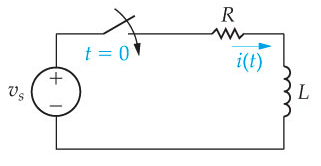
\includegraphics[width=0.4\textwidth]{9.10 Circuit.png}
    \end{figure} \\
    \textbf{Select the correct expression for $i(t)$ for $t \ge 0$.} \\
    convert the circuit to the frequency domain,
    \begin{align*}
        \textbf{V} &= 20 \phase{25^{\circ}} \\
        \textbf{Z} &= R + j \omega L\ \Omega \\
                   &= 80 + j(800)(75*10^{-3})\ \Omega \\
                   &= 80 + 60\ \Omega \\
                   &= 100 \phase{36.87^{\circ}}
    \end{align*}
    from Ohm's Law
    \[
        I = \frac{V}{R}
    ,\]
    and in the frequency domain,
    \[
        \textbf{I} = \frac{\textbf{V}}{\textbf{Z}}
    .\]
    With this the current can be found to be,
    \begin{gather*}
        \textbf{I} = \frac{20 \phase{25^{\circ}}}{100 \phase{36.87^{\circ}}} =
        0.2 \phase{-11.8699^{\circ}}\ A \\
        \boxed{i(t) = 200 \cos (800 t - 11.9^{\circ}\ mA}
    \end{gather*}
    \section*{Problem 9.13}
    A $350\ Hz$ sinusoidal voltage with a maximum amplitude of $90\ V$ at $t =
    0$ is applied across the terminals of an inductor. The maximum amplitude of
    the steady-state current in the inductor is $20\ A$. \\
    \textbf{If the phase angle of the voltage is zero, what is the phase angle
    of the current?} \\
    \par Since the current of the voltage is zero and the circuit is purely
    inductive, the angle of the current will be lagging by $90^{\circ}$
    \[
        \boxed{\theta_{i} = -90^{\circ}}
    .\]
    \textbf{What is the inductive reactance of the inductor?}
    \begin{gather*}
        \frac{90\ V}{\omega L} = 20\ A \\
        \omega L = \frac{90}{20} = \boxed{4.5\ \Omega}
    \end{gather*}
    \textbf{What is the inductance of the inductor?}
    \begin{gather*}
        \omega L = 4.5\ \Omega \\
        \omega = 2 \pi (350) \\
        L = \frac{4.5}{\omega} =  0.002046\ H = \boxed{2.05\ mH}
    \end{gather*}
    \textbf{What is the impedance of the inductor?}
    \begin{gather*}
        j \omega L = j (4.5)\ \Omega \\
        \boxed{Z_{L} = 0 + j4.5\ \Omega}
    \end{gather*}
    \section*{Problem 9.15}
    A $50\ \Omega$ resistor, a $5\ mH$ inductor, and a $1.25\ \mu F$ capacitor
    are connected in series. The series-connected elements are energized by a
    sinusoidal voltage source whose voltage is $600 \cos (8000 t + 20^{\circ})\
    V$. \\
    \textbf{Determine the impedances of the elements in the frequency-domain
    equivalent circuit.}
    \begin{gather*}
        Z_{R} = R = \boxed{50\ \Omega} \\
        Z_{L} = j \omega L = j (8000) (5*10^{-3}) = \boxed{j 40\ \Omega} \\
        Z_{C} = \frac{-j}{\omega C} = \frac{-j}{(8000)(1.25*10^{-6})} =
        \boxed{-j 100 \Omega}
    \end{gather*}
    \textbf{Reference the current in the direction of the voltage rise across
    the source, and find the phasor current.}
    \begin{gather*}
        Z_{eq} = (50 + j 40 + -j 100)\ \Omega = 50 - j 60\ \Omega = 78.1025
        \phase{-50.19}\ \Omega \\
        \textbf{I} = \frac{\textbf{V}}{\textbf{Z}} = \frac{600
        \phase{20^{\circ}}}{78.1025 \phase{-50.19}} = \boxed{7.68 \phase{70.19}\
        A}
    \end{gather*}
    steady state expression for the current:
    \[
        \boxed{i(t) = 7.68 \cos (8000 t + 70.2^{\circ})\ A}
    \]
    \section*{Problem 9.17}
    Three branches having impedances of $3 + j 4\ \Omega$, $16 - j 12\ \Omega$,
    and $-j 4\ \Omega$, respectively, are connected in parallel. \\
    \textbf{What is the equivalent admittance of the parallel connection?}
    \begin{gather*}
        Y_{ab} = \frac{1}{Z_{ab}} \\
        Y_{ab} = \frac{1}{3 + j 4} + \frac{1}{16 - j 12} + \frac{1}{-j 4} \\
        \textbf{Y}_{ab} = 0.16 + j 0.12 = \boxed{0.2 \phase{36.87^{\circ}}\ S}
    \end{gather*}
    Conductance of the parallel connection: $\boxed{0.16\ S}$ \\
    Susceptance of the parallel connection: $\boxed{0.12\ S}$
    \newpage
    \noindent\textbf{If the parallel branches are excited from a sinusoidal
    current source where $i(t) = 4 \cos (\omega t)\ A$, what is the maximum
    amplitude of the current in the purely capacitive branch?}
    \begin{gather*}
        \textbf{V} = \frac{\textbf{I}}{\textbf{Y}} = \frac{4
        \phase{0^{\circ}}}{0.2 \phase{36.87^{\circ}}} = 20
        \phase{-36.87^{\circ}}\ V \\
        \textbf{I}_{C} = \frac{\textbf{V}}{\textbf{Z}_{C}} = \frac{20
        \phase{-36.87^{\circ}}}{4 \phase{-90^{\circ}}} = 5 \phase{53.12^{\circ}}
        \\
        \boxed{\textbf{I}_{C} = 5\ A}
    \end{gather*}
    \section*{Problem 9.30}
    \begin{figure}[h]
        \centering
        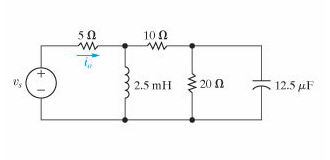
\includegraphics[width=0.6\textwidth]{9.30 Circuit.png}
    \end{figure}
    \noindent \textbf{Find $i_{0}(t)$ if $v_{s} = 45 \sin (4000 t)\ V$. Suppose
    that $i_0(t) = I_{0} \cos (\omega t + \phi)$, where $-360^{\circ} < \phi \le
    360^{\circ}$. Determine the values $I_0$, $\omega$, and $\phi$.} \\
    Converting to the frequency domain,
    \begin{gather*}
        v_{s} = 45 \sin (4000 t) = 45 \cos (4000 t - 90^{\circ}) = 45
        \phase{-90^{\circ}} \\
        Z_{C} = \frac{-j}{(4000) (12.5*10^{-6})} = -j 20\ \Omega \\
        Z_{L} = j (4000) (2.5*10^{-3}) = j 10\ \Omega
    \end{gather*}
    Now to compute the equivalent impedance seen by $v_{s}$:
    \begin{gather*}
        20\ \Omega\ || -j 20 \Omega = 10 - j 10\ \Omega \\
        10\ \Omega + (10 - j 10)\ \Omega = 20 - j 10\ \Omega \\
        (20 - j 10)\ \Omega\ ||\ j 10\ \Omega = 5 + j 10\ \Omega \\
        5 + (5 + j 10) = 10 + j 10\ \Omega \\
        Z_{eq} = 10 + j 10\ \Omega
    \end{gather*}
    Now,
    \begin{gather*}
        \textbf{I} = \frac{\textbf{V}}{\textbf{Z}_{eq}} = \frac{45
        \phase{-90^{\circ}}}{10 + j 10} = \frac{45 \phase{-90^{\circ}}}{14.14214
        \phase{45^{\circ}}} \\
        \textbf{I} = 3.18198 \phase{-135^{\circ}} \\
        \boxed{I_0 = 3.18\ A,\ \omega = 4000\ rad / s,\ \phi = -135^{\circ}}
    \end{gather*}
    \section*{Problem 9.25}
    Find the admittance $Y_{ab}$ in the circuit seen in figure 1. Take that
    $R_1 = 7\ \Omega$, $R_2 = 4\ \Omega$, $R_3 = 7\ \Omega$, and $R_4 = 12.2\
    \Omega$.
    \begin{figure}[h]
        \centering
        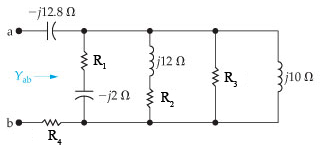
\includegraphics[width=0.6\textwidth]{9.25 Circuit.png}
    \end{figure}
    \textbf{Express $Y_{ab}$ in rectangular form.}
    \begin{gather*}
        Y_1 = \frac{1}{j 10} + \frac{1}{7} + \frac{1}{4 + j 12} + \frac{1}{7 - j
        2} = 0.2999 - j 0.1373\ S \\
        Z_1 = \frac{1}{Y_1} = \frac{1}{0.2999 - j 0.1373} = 2.7567 + j 1.2616\
        \Omega \\
        Z_{ab} = Z_1 + 4 - j 12.8 = 6.767 - j 11.5384 \\
        Y_{ab} = \frac{1}{Z_{ab}} = 0.0378 + j 0.0645\ S \\
        \boxed{Y_{ab} = 37.8 + j 64.5\ mS}
    \end{gather*}
    \newpage
    \section*{Problem 9.27}
    Consider the circuit shown. Suppose $R = 110\ \Omega$, $L = 130\ \mu H$, and
    $C = 30\ nF$.
    \begin{figure}[h]
        \centering
        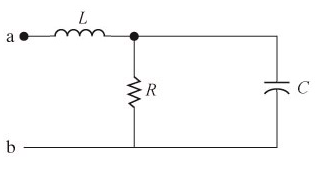
\includegraphics[width=0.4\textwidth]{9.27 Circuit.png}
    \end{figure}
    \\
    \textbf{Find the frequency (in radians per second) at which the impedance
    $Z_{ab}$ is purely resistive.}
    \begin{gather*}
        Z_{C} = \frac{-j}{\omega C} = \frac{-j}{\omega (30*10^{-9})} \\
        Z_{L} = j \omega L = j \omega (130*10^{-6}) \\
        Z_{ab} = Z_{L} + (R || Z_{C}) =  j \omega L + \frac{-jR / \omega C}{R -
        j / \omega C} \\
        Z_{ab} = j \omega L + \frac{-jR}{\omega C R - j} = j \omega L +
        \frac{-jR(\omega CR + j)}{\omega^2 C^2 R^2 + 1} \\
    \end{gather*}
    Now,
    \begin{gather*}
        \omega L - \frac{\omega C R^2}{\omega^2 C^2 R^2 + 1} = 0 \\
        L = \frac{C R^2}{\omega C^2 R^2 + 1} \\
        \omega^2 C^2 R^2 + 1 = \frac{C R^2}{L} \\
        \omega = \sqrt{\frac{C R^2 / L - 1}{C^2 R^2}} = \boxed{4.06*10^{5}\ rad
        / s}
    \end{gather*}
    \textbf{Find the value of $Z_{ab}$ at the frequency of Part A.}
    \begin{gather*}
        Z_{ab} = j \omega L + \frac{-jR}{\omega C R - j} \\
        Z_{ab} = \boxed{39.4\ \Omega}
    \end{gather*}
    \section*{Problem 9.48}
    Find the Norton equivalent with respect to terminals $a$ and $b$ in the
    circuit. Suppose that $R = 20\ \Omega$.
    \begin{figure}[h]
        \centering
        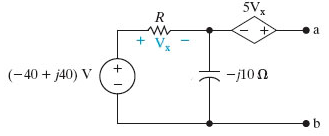
\includegraphics[width=0.5\textwidth]{9.48 Circuit.png}
    \end{figure}
    \\
    \textbf{Find the value of I$_{N}$.} \\
    Since the Norton's current is the short circuit current,
    \begin{gather*}
        -v_{s} + Ri_1 + -j 10 (i_1 - I_N) = 0 \\
        -5 V_{x} + -j 10 (I_N - i_1) = 0 \\
        V_{x} = R i_1 = 20 i_1
    \end{gather*}
    Solving for $I_{N}$:
    \[
        \boxed{I_{N} = 5.5 + j 4.5\ A}
    \]
    \textbf{Find the value of $Z_{N}$.}
    \begin{gather*}
        Z_{N} = \frac{V_{oc}}{I_{N}} \\
        i_1 = \frac{v_{s}}{20 - j 10} = -2.4 + j 0.8\ A \\
        V_{x} = -48 + j 16\ V \\
        V_{oc} = 5 V_{x} - j 10 i_1 = -232 + j 104\ V
    \end{gather*}
    Finally,
    \begin{gather*}
        Z_{N} = \frac{V_{oc}}{I_{N}} = \frac{-232 + j 104}{5.5 + j 4.5} \\
        \boxed{Z_{N} = -16 + j 32\ \Omega}
    \end{gather*}
    \newpage
    \section*{Problem 9.49}
    Find the Norton equivalent circuit with respect to the terminals $a$ and $b$
    for the circuit where $\textbf{V}_{s} = 5 \phase{0^{\circ}}\ V$ and $R =
    100\ \Omega$.
    \begin{figure}[h]
        \centering
        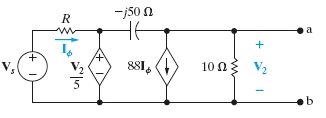
\includegraphics[width=0.5\textwidth]{9.49 Circuit.png}
    \end{figure}
    \\
    \textbf{Find the value of I$_{N}$.} \\
    Since the Norton's current is the short circuit current, putting a wire
    along the terminals $a$ and $b$ will lead to $V_2$ being zero since there is
    no voltage along the $10\ \Omega$ resistor. This shuts off the dependant
    voltage source and shunts the resistor.
    \begin{figure}[h]
        \centering
        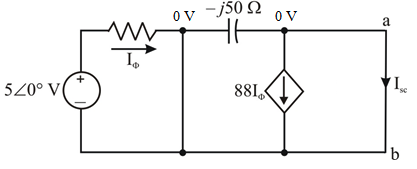
\includegraphics[width=0.5\textwidth]{9.49 Simplified Circuit.png}
    \end{figure}
    \\
    \noindent Both of the nodes, on the left and the right, are at zero volts
    since they are directly connected to ground.
    \begin{gather*}
        -I_{\phi} = \frac{0-5}{R} = \frac{-5}{100} = -0.05\ A \\
        I_{\phi} = 0.05\ A
    \end{gather*}
    At node 2,
    \begin{gather*}
        \frac{0-0}{-j 50} + 88 I_{\phi} + I_{N} = 0 \\
        88(0.05) + I_N = 0 \\
        \boxed{I_N = -4.4\ A}
    \end{gather*}
    \textbf{Find the value of Z$_{N}$.} \\
    The value of $V_{oc} = V_{TH} = V_2$ must be found from which the equivalent
    impedance can be calculated.
    \\
    The node above the current source and the resistor are the same node and its
    equation,
    \begin{gather*}
        \frac{V_2 - V_2 / 5}{-j 50} + 88 I_{\phi} + \frac{V_2}{10} = 0
    \end{gather*}
    Since,
    \[
        I_{\phi} = \frac{V_{s}- V_2 / 5}{100}
    ,\]
    \[
        \frac{5V_2 - V_2}{-j 250} + 88 \left( \frac{V_{s}-V_2 / 5}{100} \right)
        + \frac{V_2}{10} = 0
    .\]
    Solving for $V_2$,
    \begin{gather*}
        \frac{4V_2}{-j 250} + 88 \left( \frac{25 - V_2}{500} \right) +
        \frac{V_2}{10} = 0 \\
        \left( \frac{4}{-j 250} - \frac{88}{500} + \frac{1}{10} \right) V_2 =
        \frac{2200}{500} \\
        V_2 = -55.4377 - j 11.671\ V.
    \end{gather*}
    Now to use Ohm's Law to find $Z_{N}$,
    \begin{align*}
        Z_{N} &= \frac{V_{oc}}{I_{sc}} = \frac{V_{TH}}{I_N} \\
        Z_{N} &= \frac{-55.4377- j 11.671}{-4.4} \\
        Z_{N} &= \boxed{12.599 + j 2.653\ \Omega}
    \end{align*}
\end{document}
